\chapter{Introduction} \label{sec:intro}
Due to environmental concerns and availability of fossil fuels, the efficiency of civil aeroengines have continuously been improved over the last few decades. To improve efficiency, aeroengines have adopted high bypass ratio (BPR) \cite{Cumpsty2015}, which is supported by the increasing nacelle for bypass air and larger fan diameter. The open rotor concept takes this further by putting the fan outside of the nacelle, which may reduce fuel consumptions and carbon emissions by 10-20\% \cite{Farokhi2020} while producing more thrust than existing engines. 

However, aeroengine nacelles are designed to suppress the fan-generated noise, so this concept exposes it directly into the atmosphere, causing high noise pollution. An investigation of this noise generation and its propagation is required to develop methods to suppress this sound. In this work, a hybrid approach between the Ffowcs Williams-Hawkings (FW-H) method and CFD will be used to predict the noise generation and propagation. 

This progress report outlines the development and validation of the analytical FW-H code for monopole and dipole sources. As outlined in the initial project Gantt Chart, the preliminary code development and validation phases are currently on schedule, which allows the transition toward CFD model development in the upcoming weeks.

\section{Project Plan and Current Objectives} \label{subsec:plan}
In the Project Plan report, it was outlined that during the current term, the main objective was the development and  validation of the FW-H code, as shown in Figure \ref{fig:GC}. CFD-related tasks were also outlined for this term, however, these were deferred to focus on the code. This is done to control the input sources to prescribed mathematical functions for code validation.

Therefore, the objective of the current part of the work is to develop and validate the FW-H code by itself. Analytical inputs were used to validate the accuracy of the phase, amplitude, and directivity pattern predictions without CFD data. 

\begin{figure}[H]
    \centering
    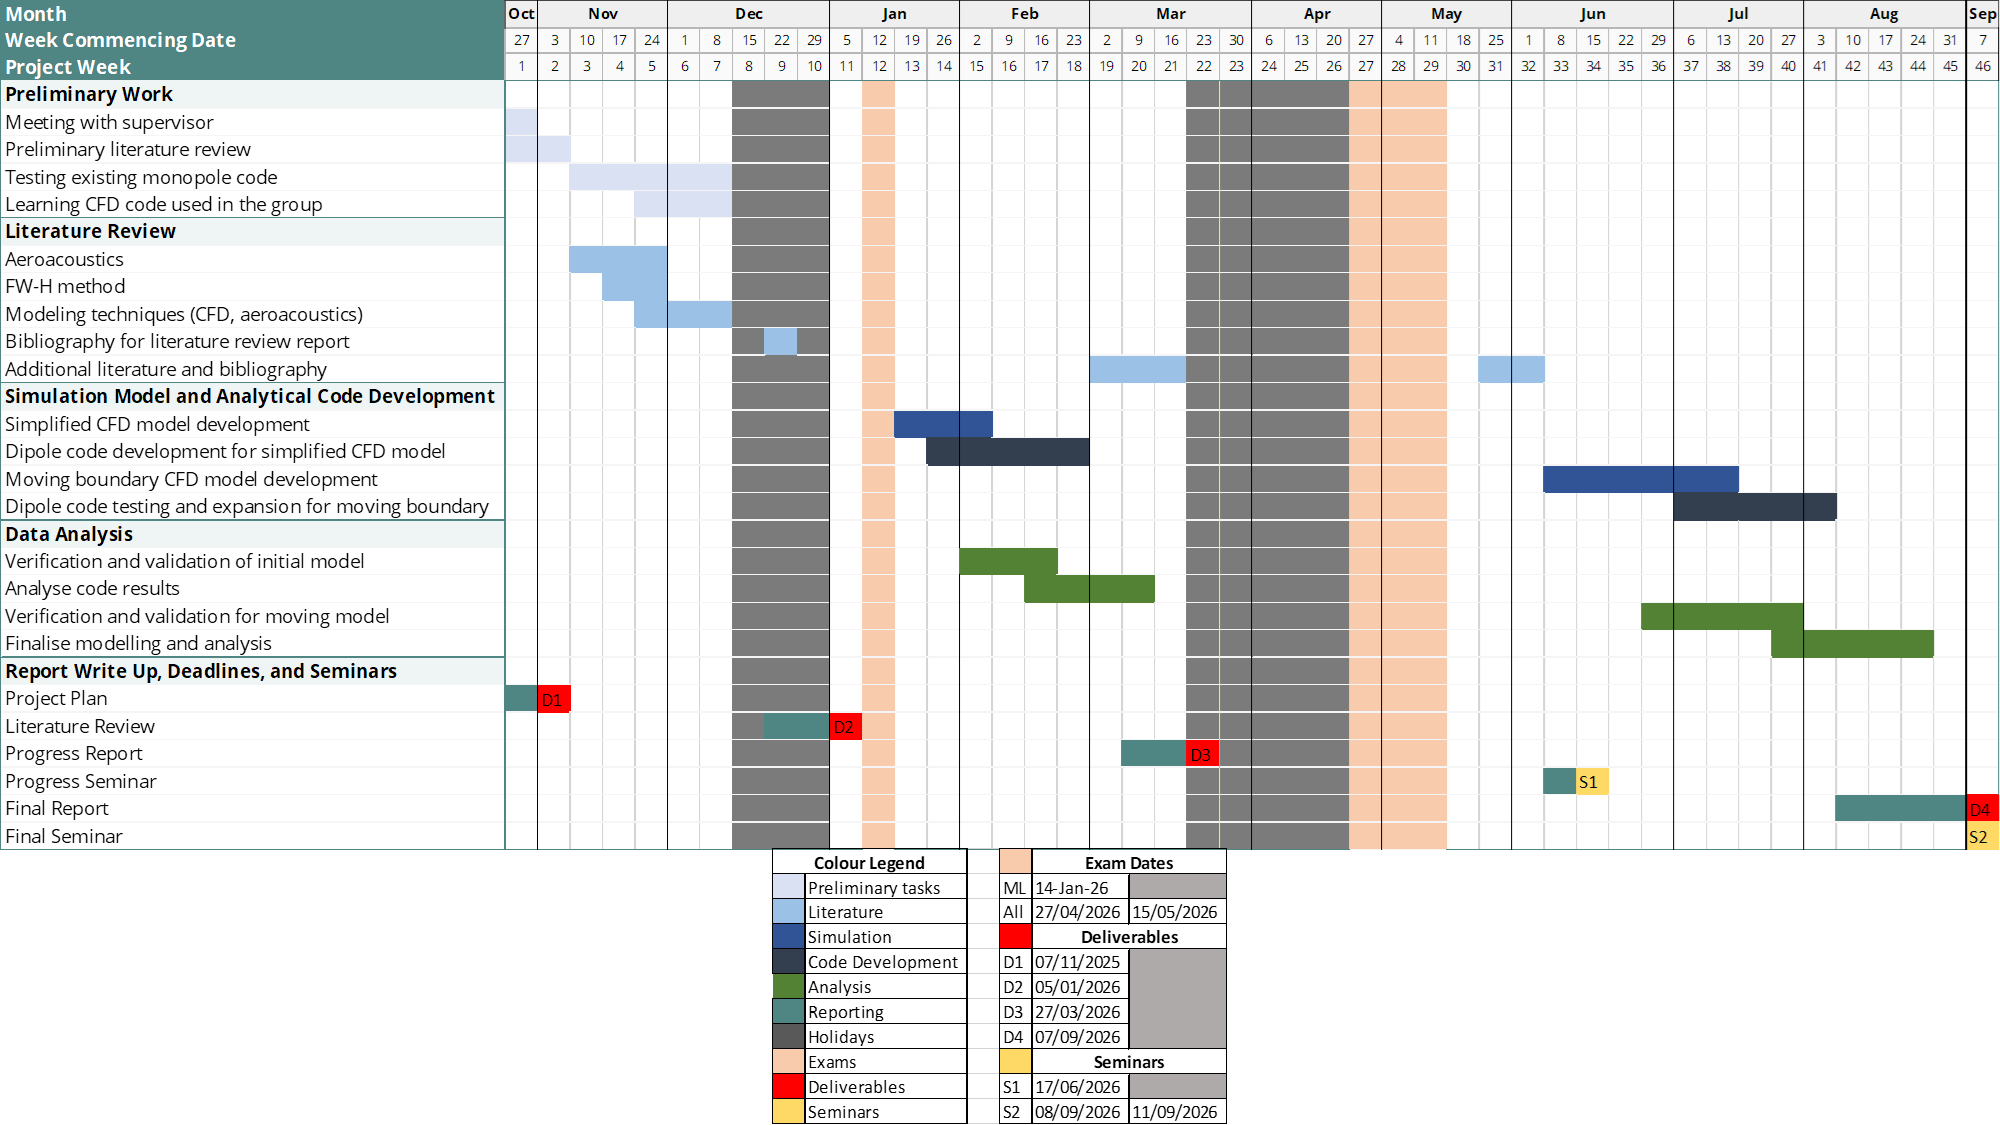
\includegraphics[width=1\linewidth]{fig_past_reports/gantt_chart.png}
    \caption{Gantt Chart of the research project}
    \label{fig:GC}
\end{figure}